\chapter{Calcul différentiel}

\section{Introduction~: Une petite balade\textellipsis}
Les fonctions apparaissent comme l'un des outils les plus proéminent des mathématiques, car elles permettent de caractériser l'évolution d'une quantité au cours d'une seconde quantité de référence. Ainsi en physique peut-on observer l'évolution d'un voltage au cours du temps, ou en chimie l'évolution d'une conductivité en fonction d'un volume d'apport. 

Pour comprendre ce qu'est le calcul différentiel et construire une intuition mathématique, il est utile de conserver en tête un problème concret.

Imagine que tu veuilles faire une randonnée de $13$ km avec tes amis mais que certains d'entre eux ne sont pas très habitués à marcher. Ainsi, tu veux éviter de prendre un trajet trop escarpé. Pour ce faire, tu déniches un site Internet qui te donne l'altitude selon la longueur du trajet déjà parcouru (c'est un site bizarre mais bien utile pour notre exemple). En réalité, tout que fait ce site est de te donner l'expression d'une fonction $f : [0, 13] \to \mathbb{R}^{+}$, que l'on va étudier plus attentivement pour savoir si le chemin est praticable ou non.

\subsection{Taux d'accroissement moyen}
Une première approche pour savoir si le chemin est trop raide est de regarder l'altitude de départ et celle d'arrivée. Puis, de la même manière que l'on calcule la \emph{vitesse moyenne}, on peut calculer le dénivelé moyen. Après quelque recherches, tu trouves les renseignements suivants (Figure \ref{fig:differential_calculus_ex_table_1})~:

\begin{table}[H]
\centering
\rowcolors{2}{lightgray!40}{lightgray!80}
\begin{tabular}{|p{10cm}|p{4cm}|}
    \hline
    Catégorie & Valeur \\
    \hline

    Altitude au début de la randonnée ($f(0)$) & 2200 m \\
    Altitude à fin de la randonnée ($f(13)$) & 2240 m \\
    Longueur du trajet & 13 km \\
    Temps estimé & 2h30 \\
    
    \hline
\end{tabular}
\caption{Information sur la randonnée prévue pour le 13.09.2023}
\label{fig:differential_calculus_ex_table_1}
\end{table}

Le dénivelé moyen est défini comme le dénivelé total divisé par la longueur du trajet. Ainsi, le dénivelé total est $\Delta A = 2240 \mathrm{m} - 2200 \mathrm{m}$ tandis que le dénivelé moyen est 
\begin{align*}
    \frac{\Delta A}{\Delta d} = \frac{2240 \mathrm{m} - 2200 \mathrm{m}}{13 \mathrm{ km}} = \frac{40 \mathrm{ m}}{13 \mathrm{ km}} \approx 2.3 \mathrm{ m}/\mathrm{km}
\end{align*}
Cela signifie que en moyenne, le chemin monte de 2.3 mètres tous les kilomètres. Ainsi, il apparaît a priori que le chemin n'est pas très escarpé. 


\smallskip

Grâce à cet exemple on peux mieux comprendre la notion de \emph{taux d'accroissement} telle que définie en mathématiques~:
\begin{boxdef}[Taux d'accroissement]
Soit $f : \mathbb{R} \to \mathbb{R}$ une fonction réelle, on définit le \emph{taux d'accroissement} de $f$ entre $a$ et $b$ comme~:
\begin{align*}
    \frac{\Delta f}{\Delta x} = \frac{f(b) - f(a)}{b - a}
\end{align*}
\end{boxdef}
Ici le $a$ et $b$ correspondent à la position de départ et de fin, respectivement. Ainsi, le $f(b) - f(a)$ correspondrait dans notre exemple au dénivelé total accumulé (altitude de fin - altitude de départ). Nous voulons une moyenne sur le chemin donc on divise par la taille de l'intervalle ($b - a$). La Figure \ref{fig:differential_calculus_figure_plot_1} donne une interprétation plus graphique~:
\begin{figure}[H]
    \centering
    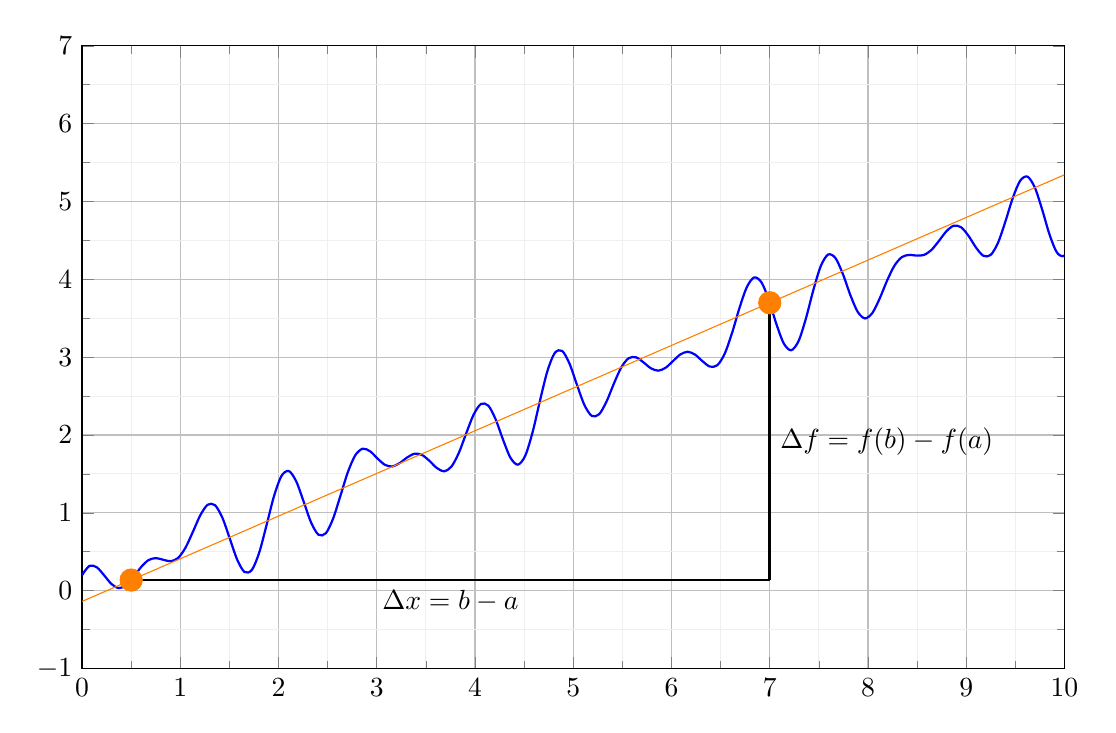
\begin{tikzpicture}
    \begin{axis}[
        xmin = 0, xmax = 10,
        ymin = -1, ymax = 7,
        xtick distance = 1,
        ytick distance = 1,
        grid = both,
        minor tick num = 1,
        major grid style = {lightgray},
        minor grid style = {lightgray!25},
        width = 400,
        height = 270,
        legend cell align = {left},
        legend pos = north west
    ]
    
    \addplot[
        domain = 0:30,
        samples = 400,
        smooth,
        thick,
        blue,
    ] {0.5*x + 0.3 * sin(387*x) - 0.1 * cos(180 * x) + 0.3 * cos(523*x)};
    
    \addplot[domain = 0:30, samples = 100, smooth, orange, width = 3pt]{0.5481377*x-0.1384454};
    
    \addplot[orange, only marks, mark size = 4pt] table {
        0.5 0.1356234
        7 3.6985189
    };
    
    \draw[line width=1pt, black] (axis cs:7,0.1356234) -- node[right]{$\Delta f = f(b) - f(a)$} (axis cs:7,3.6985189);
    
    \draw[line width=1pt, black] (axis cs:0.5,0.1356234) -- node[below]{$\Delta x = b - a$} (axis cs:7,0.1356234);
    
    \end{axis}
    \end{tikzpicture}
    \caption{Interprétation graphique du taux d'accroissement}
    \label{fig:differential_calculus_figure_plot_1}
\end{figure}

\subsection{Point dérivé}
Par l'analyse faite jusqu'à présent, le chemin que tu comptes prendre semble plus que praticable et ne risque pas de poser problème pour tes amis. Pourtant, un doute subsiste dans ton esprit car tu te souviens qu'un passage est particulièrement escarpé. En plus, tu n'est pas sans ignorer que le dénivelé moyen (et le taux d'accroissement) peut cacher un dénivelé très important sur certain passage\textellipsis

Le passage difficile se situe à $12$ km du départ et tu décides donc de récolter plus de données autour de ce kilométrage (Figure \ref{fig:differential_calculus_ex_table_2}).

\begin{table}[H]
\centering
\begin{tabular}{|p{10cm}|p{4cm}|}
    \hline
    Kilométrage & Altitude \\
    \hline

    $11$ km & $2240$ m \\
    $12$ km & $2253$ m \\
    $13$ km & $2240$ m \\
    
    \hline
\end{tabular}
\caption{Altitudes autour du $18$-ième kilomètre}
\label{fig:differential_calculus_ex_table_2}
\end{table}

De nouveau, on peux calculer le taux d'accroissement mais cette fois-ci entre le $11$-ième kilomètre et le $12$-ième kilomètre. Tu obtiens un dénivelé de $12\,\textrm{m}/\textrm{km}$. Tu décides de prendre sur Internet un cliché de cette zone (Figure \ref{fig:differential_calculus_ex_table_3}).

\begin{figure}[H]
    \centering
    \includegraphics[width=0.7\textwidth]{assets/imgs/banniere-0331.jpg}
    \caption{Pourquoi le dénivelé moyen c'est pas fou}
    \label{fig:differential_calculus_ex_table_3}
\end{figure}

On est confronté ici avec l'une des limitations du taux d'accroissement~: il s'agit d'une valeur \emph{moyenne} et donc on perd, dans une certaine mesure, l'information très locale du parcours. En effet, on sait uniquement que l'altitude au $11$-ième kilomètre est de $2253$m et devient $2265$m au $12$-ième km. En d'autre termes, on est incapable de différentier les deux courbes suivantes au seul taux d'accroissement (Figure \ref{fig:differential_calculus_figure_plot_4}) :


\begin{figure}[H]
    \centering
    \begin{subfigure}[b]{0.45\textwidth}
         \centering
         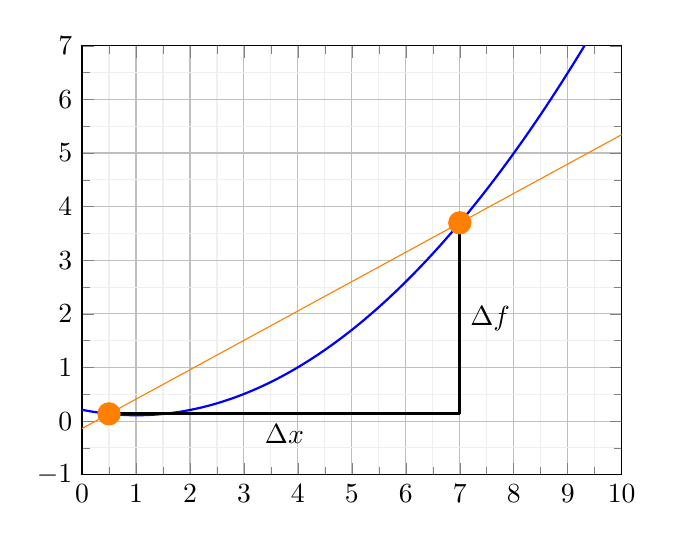
\begin{tikzpicture}
            \begin{axis}[
                xmin = 0, xmax = 10,
                ymin = -1, ymax = 7,
                xtick distance = 1,
                ytick distance = 1,
                grid = both,
                minor tick num = 1,
                major grid style = {lightgray},
                minor grid style = {lightgray!25},
                width = 240,
                height = 200,
                legend cell align = {left},
                legend pos = north west
            ]
            
            \addplot[
                domain = 0:30,
                samples = 400,
                smooth,
                thick,
                blue,
            ] {0.5481377*x-0.1384454 + (x - 0.5) * (x - 7) * 0.1};
            
            \addplot[domain = 0:30, samples = 100, smooth, orange, width = 3pt]{0.5481377*x-0.1384454};
            
            \addplot[orange, only marks, mark size = 4pt] table {
                0.5 0.1356234
                7 3.6985189
            };
            
            \draw[line width=1pt, black] (axis cs:7,0.1356234) -- node[right]{$\Delta f$} (axis cs:7,3.6985189);
            
            \draw[line width=1pt, black] (axis cs:0.5,0.1356234) -- node[below]{$\Delta x$} (axis cs:7,0.1356234);
            
            \end{axis}
         \end{tikzpicture}
         \caption{Une rando sympa}
         \label{fig:aergfpiegrbpiaergbpuiaerg}
     \end{subfigure}
     \hfill
     \begin{subfigure}[b]{0.45\textwidth}
         \centering
         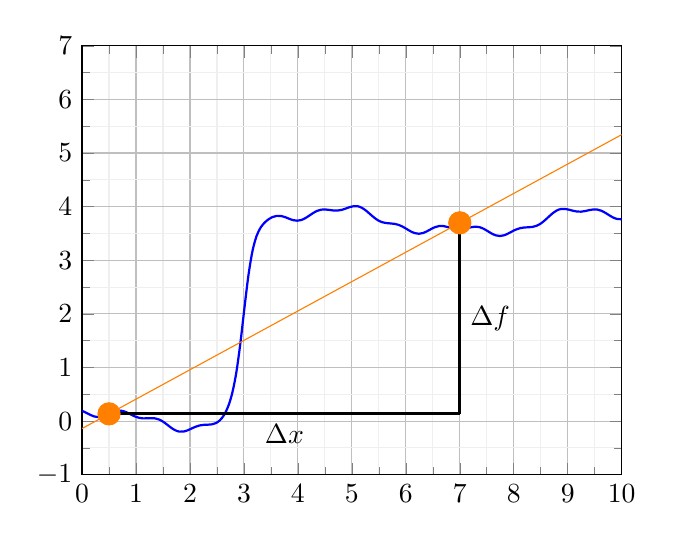
\begin{tikzpicture}
            \begin{axis}[
                xmin = 0, xmax = 10,
                ymin = -1, ymax = 7,
                xtick distance = 1,
                ytick distance = 1,
                grid = both,
                minor tick num = 1,
                major grid style = {lightgray},
                minor grid style = {lightgray!25},
                width = 240,
                height = 200,
                legend cell align = {left},
                legend pos = north west
            ]
            
            
            \addplot[
                domain = 0:30,
                samples = 400,
                smooth,
                thick,
                blue,
            ] {0.1356234 + (3.6985189 - 0.1156234) / (1 + e^(-10*(x - 3))) + 0.1 * sin(180 * (x - 0.5)) - 0.2 * sin(68 * (x - 0.5)) + 0.05 * sin(486 * (x - 0.5))};
            
            \addplot[domain = 0:30, samples = 100, smooth, orange, width = 3pt]{0.5481377*x-0.1384454};
            
            \addplot[orange, only marks, mark size = 4pt] table {
                0.5 0.1356234
                7 3.6985189
            };
            
            \draw[line width=1pt, black] (axis cs:7,0.1356234) -- node[right]{$\Delta f$} (axis cs:7,3.6985189);
            
            \draw[line width=1pt, black] (axis cs:0.5,0.1356234) -- node[below]{$\Delta x$} (axis cs:7,0.1356234);
            
            \end{axis}
         \end{tikzpicture}
         \caption{Une rando pas sympa}
         \label{fig:three sin x}
     \end{subfigure}
    \caption{Interprétation graphique du taux d'accroissement}
    \label{fig:differential_calculus_figure_plot_4}
\end{figure}

On cherche une notion plus raffinée pour caractériser l'accroissement très local, ce que l'on obtient par le \emph{dénivelé instantané}, qui nous permet savoir si en un point du trajet la route est escarpé ou non. Ce dénivelé instantané représenterait le dénivelé en un point. Autrement dit, on veux un taux d'accroissement mais qui caractérise l'accroissement en un seul point (au lieu de l'accroissement entre deux points). Pour ce faire, on va rapprocher les deux valeurs $a$ et $b$, de telle sorte à ce qu'elles deviennent infiniment proches, à travers la notion de \emph{limite}. On appelle ainsi le résultat de cette procédure la \emph{dérivée} en un point~:
\begin{boxdef}[Fonction dérivée]
    Soit $f : \mathbb{R} \to \mathbb{R}$ une fonction réelle. La \emph{dérivée} de cette fonction au point $a \in \mathbb{R}$ est définie par
    \begin{equation}
    f'(a) = \lim_{b \to a} \frac{f(b) - f(a)}{b - a}
    \end{equation}
    si la limite existe.
    Par le changement de variable $h = b - a$, on obtient la définition équivalente~:
    \begin{equation}
    f'(a) = \lim_{h \to 0} \frac{f(a + h) - f(a)}{h}
    \end{equation}
\end{boxdef}

La dérivée comme nous l'avons définie nous permet alors de représenter la pente en un point. Ainsi, si le dénivelé instantané est positif, alors la suite du chemin nous fait monter en altitude, et inversement. Ceci explique le lien entre \emph{signe de la dérivée} et \emph{monotonie} d'une fonction~:
\begin{boxthm}[Lien entre monotonie et signe de la dérivée]
    Soit $f : D \to \mathbb{R}$ une fonction réelle dérivable sur un intervalle $I \subseteq D$, telle que $f'(x) \geq 0$ (respectivement $f'(x) \leq 0$) pour tout $x \in I$. Alors la fonction $f$ est croissante (respectivement décroissante) sur $I$.
\end{boxthm}
Notons que le cas particulier $f'(x) = 0$ implique que $f$ est à la fois croissante et décroissante sur l'intervalle $I$, c'est-à-dire que $f$ est une fonction constante sur $I$.

% Plus adapté pour des exercices à mon avis
% \textbf{\underline{Exemple numérique :}}

% Trouvez la dérivé des fonctions $f(x)$ suivantes en utilisant uniquement la définition
% \begin{enumerate}
%     \item $f(x) = x^2$
%     \item $f(x) = \cos(x)$
% \end{enumerate}

% \vspace{5mm}

% \begin{enumerate}
%     \item $f(x) = x^2$ 
    
%     \vspace{2mm}
    
%     Par la définition on a:
%     \begin{align*}
%         f'(x) &= \lim_{h \to 0} \frac{f(x + h) - f(x)}{h} \\
%         &= \lim_{h \to 0} \frac{(x + h)^2 - x^2}{h} \\
%         &= \lim_{h \to 0} \frac{x^2 + 2xh + h^2 - x^2}{h} \\
%         &= \lim_{h \to 0} 2x + h \\
%         &= 2x
%     \end{align*}
    
%     \vspace{2mm}
    
%     \item $f(x) = \cos(x)$
    
%     \vspace{2mm}
    
%     \begin{align*}
%         f'(x) &= \lim_{h \to 0} \frac{\cos(x + h) - \cos(x)}{h} \\
%         &= \lim_{h \to 0} \frac{\cos(x)\cos(h) - \sin(x) \sin(h) - \cos(x)}{h} \\
%         &= \lim_{h \to 0} \frac{\cos(x) (\cos(h) - 1) - \sin(x) \sin(h)}{h} \\
%         &= \lim_{h \to 0} \frac{\cos(x) (\cos(h) - 1)}{h} - \frac{\sin(x) \sin(h)}{h} \\
%         &= \cos(x) \lim_{h \to 0} \underbrace{\frac{\cos(h) - 1}{h}}_{\to 0} - \sin(x) \lim_{h \to 0} \underbrace{\frac{\sin(h)}{h}}_{\to 1} \\
%         &= - \sin(x)
%     \end{align*}
    
% \end{enumerate}


\section{Approche plus rigoureuse}
La définition précédente cache de nombreux problèmes non triviaux que l'on peux rencontrer avec les dérivées. 

Tout d'abord, une fonction n'est pas forcement définie sur $\mathbb{R}$, e.g. $f(x) = x \sqrt{x}$ n'est définit que pour $x \geq 0$. Il devient alors problématique de définir la dérivée aux bords de son ensemble de définition, par exemple quelle serait la dérivée de la fonction $f$ ci-dessus en $0$ ?\footnote{On pourrait définir dans ce cas la dérivée uniquement en considérant la limite à droite, mais si l'on considère la dérivée en termes de pente de la tangente, la tangente en $x = 0$ n'est pas proprement définie pour que la définition soit cohérente.}

Ensuite, certaines fonctions ne sont pas continues en certains points (cf. Figure \ref{fig:differential_calculus_figure_plot_5}). Puisque ces fonctions ont un saut, cela provoque la divergence de la limite en ces points. Dans la figure ci-dessous, si $f(5) = 0$, on a
\begin{equation}
\lim_{h \to 0^+} \frac{\overbrace{f(5+h)}^{=1}-f(5)}{h} = \lim_{h \to 0^+} \frac{1}{h} = \infty \quad \textrm{et} \quad \lim_{h \to 0^-} \frac{\overbrace{f(5+h)}^{=0}-f(5)}{h} = 0
\end{equation}
La dérivée n'est donc pas définie en $x = 5$. Une fonction dérivable en un point est \emph{nécessairement} continue en ce point.

\begin{figure}[H]
    \centering
    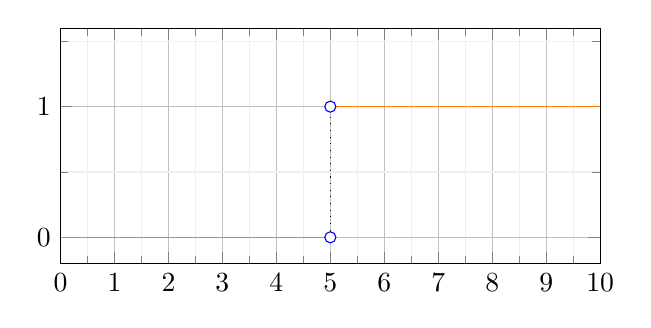
\begin{tikzpicture}
        \begin{axis}[
            xmin = 0, xmax = 10,
            ymin = -0.2, ymax = 1.6,
            xtick distance = 1,
            ytick distance = 1,
            grid = both,
            minor tick num = 1,
            major grid style = {lightgray},
            minor grid style = {lightgray!25},
            width = 240,
            height = 130,
            legend cell align = {left},
            legend pos = north west
        ]
            
            \addplot[domain = 0:5, samples = 20, smooth, orange, width = 5pt]{0};
            
            \addplot[domain = 5:10, samples = 20, smooth, orange, width = 5pt]{1};
            
            \addplot[color=blue,fill=white,only marks,mark=*] coordinates{(5,0)(5,1)};
            
            \draw[dotted] (axis cs:5,0) -- (axis cs:5,1);
                
        \end{axis}
    \end{tikzpicture}
    \caption{Exemple de discontinuité}
    \label{fig:differential_calculus_figure_plot_5}
\end{figure}
    
Enfin, la continuité \emph{n'est pas suffisante} pour assurer que fonction soit dérivable. Prenons l'exemple $f(x) = |x|$ (Figure \ref{fig:differential_calculus_figure_plot_6}) où $f : \mathbb{R} \mapsto \mathbb{R}$ et demandons nous combien $f'(0)$ vaut.
    
\begin{figure}[H]
    \centering
    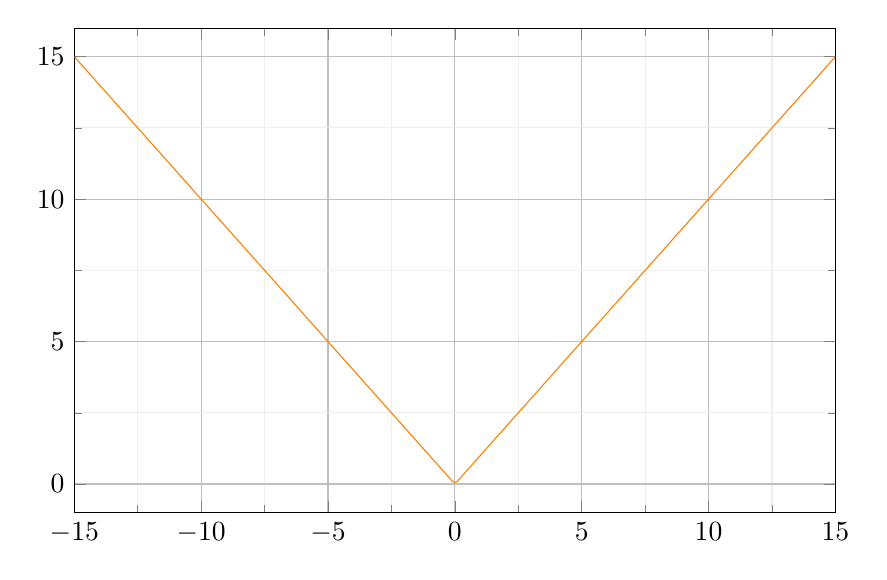
\begin{tikzpicture}
        \begin{axis}[
            xmin = -15, xmax = 15,
            ymin = -1, ymax = 16,
            xtick distance = 5,
            ytick distance = 5,
            grid = both,
            minor tick num = 1,
            major grid style = {lightgray},
            minor grid style = {lightgray!25},
            width = 320,
            height = 220,
            legend cell align = {left},
            legend pos = north west
        ]
            
            \addplot[domain = -15:15, samples = 200, smooth, orange, width = 5pt]{abs(x)};
            
        \end{axis}
    \end{tikzpicture}
    \caption{Fonction $|x|$}
    \label{fig:differential_calculus_figure_plot_6}
\end{figure}
    
Intuitivement, la dérivée correspond à l'évolution locale de la fonction. Notamment, si la dérivée est positive (respectivement négative) alors la fonction sera croissante (respectivement décroissante).

Il est clair que $f$ est continue en $0$. Le problème est le suivant~: la fonction est-telle instantanément décroissante ou croissante en $0$ ? Pour y répondre, nous pouvons agrandir la zone d'intérêt. Mais quelque soit notre niveau de zoom, le point $x = 0$ reste anguleux. Plus rigoureusement, si l'on essaie de calculer les limites à droite et à gauche, on trouve par la définition de $f(x) = |x|$ que
\begin{equation}
\lim_{h \to 0^+} \frac{f(h) - f(0)}{h} = \lim_{h \to 0^+} \frac{h}{h} = 1 \quad \textrm{et} \quad \lim_{h \to 0^-} \frac{f(h)-f(0)}{h} = \lim_{h \to 0^-} \frac{-h}{h} = -1
\end{equation}
Ainsi, les deux équations traduisent bien la contradiction qu'il y a à définir la (dé)croissance en $x = 0$.

% Je pense que ces paragraphes là ne sont pas nécessaires
% Ainsi voici une définition plus rigoureuse de la dérivabilité (existence d'une dérivé) et de la dérivée d'une fonction

% \begin{boxdef}{Dérivée et Dérivabilité}
%     Soit $f$ une fonction définie sur un intervalle ouvert $[a, b]$ à valeur dans $\mathbb{R}$. On dit que la dérivé de $f$ en $c \in ]a, b[$ (noté $f'(c)$) est la valeur de la limite suivante \textbf{si elle converge}.
    
%     \begin{align*}
%         f'(c) = \lim_{h \to 0} \frac{f(c + h) - f(c)}{h}
%     \end{align*}
    
%     Notez qu'il n'y a pas de condition d'approche sur $h$, en particulier la limite doit convergez sur la même valeur par la gauche et par la droite. \Bigg(Autrement dit $\displaystyle f'(c) = \lim_{h \to 0, \  h < 0} \frac{f(c + h) - f(c)}{h} = \lim_{h \to 0, \ h > 0} \frac{f(c + h) - f(c)}{h}$ \Bigg)
% \end{boxdef}

% \vspace{8mm}

% \textbf{\underline{Exemple~:}} 

% \vspace{1mm}

% \begin{itemize}
%     \item $f(x) = \begin{cases} 0, & x < 5 \\ 1, & x \geq 5 \end{cases}$ \quad (Figure \ref{fig:differential_calculus_figure_plot_5})
    
%     Selon la définition si dessus, la dérivé en $x = 5$ est:
    
%     \begin{align*}
%         f'(5) = \lim_{h \to 0} \frac{f(5 + h) - f(5)}{h} = \lim_{h \to 0} \frac{f(5 + h)}{h}
%     \end{align*}
%     Pour $h > 0$
%     \begin{align*}
%         f'(5) = \lim_{h \to 0} \frac{1}{h} = \infty \not \in \mathbb{R}
%     \end{align*}
    
%     Ainsi la limite ne converge pas est donc la dérivé n'existe pas
    
%     \vspace{5mm}
    
%     \item $f(x) = |x| = \begin{cases} x, & x > 0 \\ -x, & x < 0 \end{cases}$ \quad (Figure \ref{fig:differential_calculus_figure_plot_6})

%     Selon la définition on a :
%     \begin{align*}
%         f'(0) = \lim_{h \to 0} \frac{f(h) - f(0)}{h} = \lim_{h \to 0} \frac{f(h)}{h}
%     \end{align*}
    
%     \begin{itemize}
%         \item Pour $h > 0$ on a:
%         \begin{align*}
%             f'(0^+) = \lim_{h \to 0^+} \frac{f(h)}{h} = \lim_{h \to 0^+} \frac{h}{h} = 1
%         \end{align*}
        
%         \item Pour $h < 0$ on a:
%         \begin{align*}
%             f'(0^-) = \lim_{h \to 0^-} \frac{f(h)}{h} = \lim_{h \to 0^-} \frac{-h}{h} = -1
%         \end{align*}
%     \end{itemize}
    
%     Ainsi la limite par la gauche n'est pas égale celle par la droite, donc la limite ne converge pas et la fonction n'admet pas de dérivé en $x = 0$

%     \vspace{5mm}    

%     \item $f(x) = x \sqrt{x}$ définit sur $\mathbb{R}^+$ en $0$ \\
    
%     \vspace{1mm}
    
%     \textbf{Cette exemple est plus poussé que les autres et n'est pas nécessaire pour la compréhension du cours. Il s'agit d'argumenter sur un des détails de la définition (et introduire ce qu'elle omet)}
    
%     \vspace{1mm}
    
%     La définition précédente ne définit pas la dérivé en $0$ car $0$ est l'une des bornes de l'intervalle $[0, +\infty[$. Or $f'(x)$ n'est définit que sur $]0, +\infty[$. Pourquoi ne définissons nous pas la dérivé au borne de l'intervalle ?
    
%     En pratique on utilise une définition légèrement différente pour la dérivé aux bornes qui prends en compte le fait que $f(x), x < 0$ ne soit pas définit. La limite de la définition est une limite \textbf{par la gauche et par la droite} (et donc pour $h < 0$ évalue $f(x), x < 0$). Ainsi pour évalué la dérivé aux bornes on utilise la limite qui n'évalue pas la fonction en dehors de son domaine de définition. Dans ce cas particulier on évaluera~:
    
%     \begin{align*}
%         f'(0) = \lim_{h \to 0^+} \frac{h \sqrt{h} - 0 \sqrt{0}}{h} = \underbrace{\lim_{h \to 0^+} \sqrt{h}}_{\text{Bien définit}} = 0
%     \end{align*}
    
%     Donc $f'(0)$ n'est pas définit dans cette exemple
% \end{itemize}

\subsection{Propriétés des dérivées}
Utiliser à chaque fois la définition formelle et la limite pour calculer la dérivée peut se montrer éreintant, et il est plus simple dans la majorité des cas de se baser sur des dérivées usuelles. Ces propriétés sont donc utiles dans la recherche de dérivées, similairement aux propriétés de combinaison des limites de suite.

\begin{boxthm}[Propriétés de la dérivée]
% Les propriétés suivantes peuvent être prouvées à l'aide de la définition. Ces preuves ne sont donc pas fournis ici et sont laissé en exercice au lecteur (il faut vous habituer à ce genre de manoeuvre d'évasion typique)

Soit $f, g$ deux fonctions définies et dérivables en $x \in \mathbb{R}$ et soit $\alpha, \beta, \lambda \in \mathbb{R}$ des constantes. Alors~:
\begin{enumerate}
    \item $(f(x) + g(x))' = f'(x) + g'(x)$
    \item $(\lambda f(x))' = \lambda f'(x)$
    \item $(f(x)g(x))' = f'(x) g(x) + f(x) g'(x)$
    \item $\left( \frac{f(x)}{g(x)} \right)' = \frac{f'(x)g(x) - f(x)g'(x)}{g(x)^2}, \quad g(x) \neq 0$
    \item Si $f$ est dérivable en $g(x)$, alors $(f(g(x)))' = f'(g(x)) g'(x)$
\end{enumerate}
\end{boxthm}
% En particulier, la dernière propriété nous permet d'énoncer la dérivée d'une fonction \emph{réciproque}~: si $g : \mathbb{R} \to \mathbb{R}$ est une fonction dérivable en $x \in \mathbb{R}$ et inversible avec $f = g^{-1}$, alors
% \begin{equation}
% f(g(x)) = x \implies (f(g(x))' = f'(g(x)) g'(x) = 1 \quad \textrm{i.e.} \ f'(g(x)) = \frac{1}{g'(x)}
% \end{equation}
% Si on note $y = g(x) \iff x = f(y)$, on obtient la formule suivante~:
% \begin{boxthm}[Dérivée d'une fonction réciproque]
% Soit $g : D \to \mathbb{R}$ une fonction dérivable et inversible, de réciproque $f = g^{-1} : \textrm{Im}(g) \to D$. Alors $f$ est dérivable et
% \begin{equation}
% f'(y) = \frac{1}{g'(f(y))}
% \end{equation}
% \end{boxthm}

% Par exemple, le \emph{logarithme népérien} $\ln : \mathbb{R}_{> 0} \to \mathbb{R}$ est la fonction réciproque de l'exponentielle $\exp : \mathbb{R} \to \mathbb{R}_{> 0}$, et ainsi sa dérivée est donnée par le théorème ci-dessus~:
% \begin{equation}
% \ln'(y) = \frac{1}{\exp(\ln(y))} = \frac{1}{y}
% \end{equation}
% puisque la dérivée de l'exponentielle est elle-même, i.e. $\exp'(x) = \exp(x)$.

On donne ici à titre d'exemples quelques dérivées primordiales qui pourraient vous être utiles (pour le reste, vous pouvez les calculer par vous-même)~:
\begin{greybox}
\textbf{Exemples de dérivées importantes.}
\begin{itemize}
    \item $\left( x^{n} \right)' = n x^{n-1} , \quad n \in \mathbb{Z}$
    \item $\cos'(x) = -\sin(x)$
    \item $\sin'(x) = \cos(x)$
    \item $\left( \exp(x) \right)' = \exp(x)$
    \item $\left( \ln(x) \right)' = \frac{1}{x}$
\end{itemize}
\end{greybox}

\section{Applications à la recherche d'extrema}

Revenons un peu à notre randonnée. Toujours dans ce contexte, tu souhaites savoir si le chemin passe par un sommet (pour profiter d'une belle vue 360°). Plus précisément, tu cherches à déterminer à quelle distance du début se situe le sommet (pour savoir si un pique-nique y est possible). Malheureusement, le site donnant l'altitude du chemin est en maintenance. En fouillant un peu tu trouves uniquement le graphique du dénivelé instantané en fonction du kilométrage pour cette ballade (Figure \ref{fig:differential_calculus_figure_plot_7}).

\begin{figure}[H]
    \centering
    \hfill
    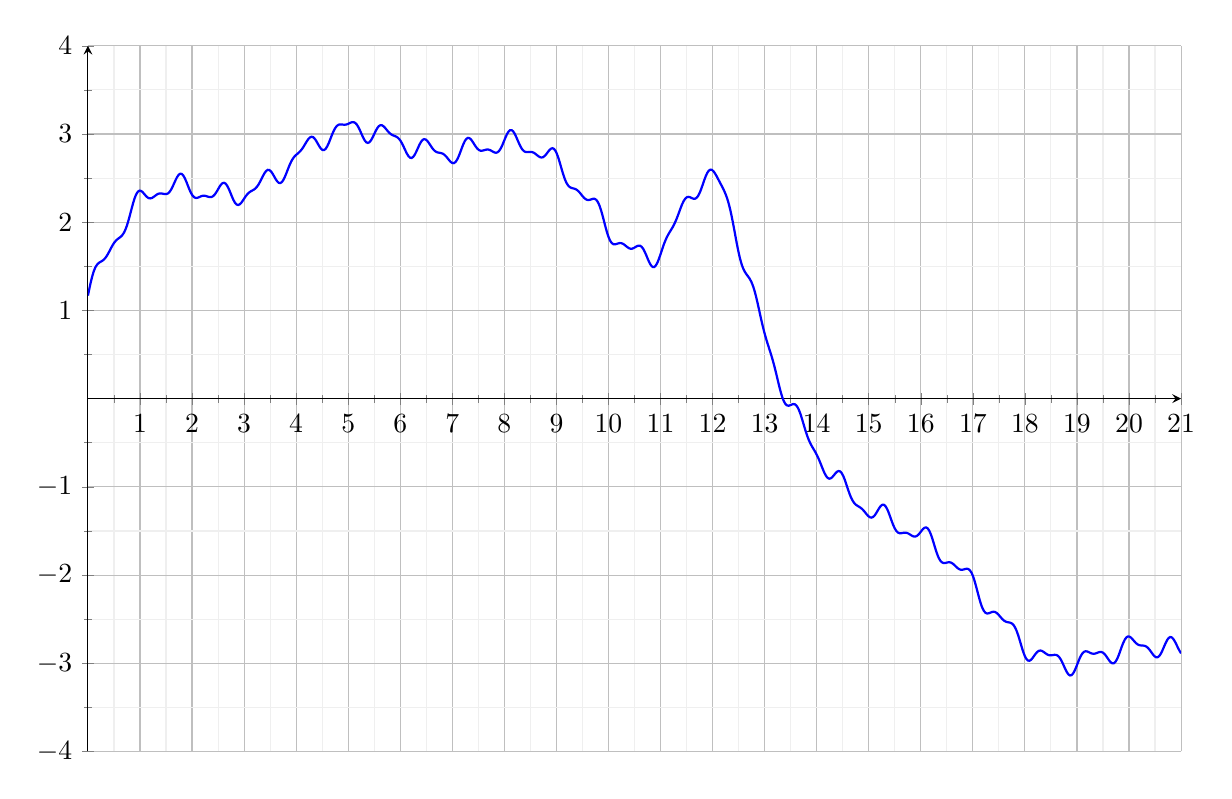
\begin{tikzpicture}
        \begin{axis}[
            xmin = 0, xmax = 21,
            ymin = -4, ymax = 4,
            xtick distance = 1,
            ytick distance = 1,
            grid = both,
            minor tick num = 1,
            major grid style = {lightgray},
            minor grid style = {lightgray!25},
            width = 440,
            height = 300,
            legend cell align = {left},
            legend pos = north west,
            axis lines=middle
        ]
            
        \addplot[
            domain = 0:21,
            samples = 700,
            smooth,
            thick,
            blue,
        ] {3 * sin(13 * x + 7) + exp(-(0.5 * (x - 1))^2) + 0.2 * sin(93*x+4) + 0.1 * sin(453*x+4) + 0.05 * sin(853*x+3) + 1.5 * exp(-(1.2 * (x - 12))^2)};
            
        \end{axis}
    \end{tikzpicture}
    \caption{Dénivelé en fonction du kilométrage}
    \label{fig:differential_calculus_figure_plot_7}
\end{figure}

Garde en tête que la Figure ci-dessus présente le dénivelé instantané (et donc la dérivée de l'altitude). Comment alors caractériser un maximum (un sommet) grâce à la dérivée ? Imagine un sommet de montagne~: on monte vers le sommet, puis une fois arrivé au sommet, on ne peux que redescendre. 

Lorsque l'on \emph{monte} (respectivement descend) le dénivelé est positif (respectivement négatif). Ainsi, un maximum est caractérisé par un changement de signe de positif à négatif, et le maximum se trouve précisément là où la dérivée est 0 (i.e. il n'y a plus de changement instantané d'altitude). Similairement, un \emph{minimum} est caractérisé par une dérivée de signe négatif, puis positif (on descend puis on monte). On observe alors l'existence d'un maximum en $x \approx 13.34889$.

Tentons ainsi de définir rigoureusement ce qu'est un \emph{maximum} ou un \emph{minimum}, i.e. ce qu'on appelle un \emph{extremum}~:

\begin{boxdef}[Extremum]
Soit $f : D \to \mathbb{R}$ une fonction réelle. On dit que $f$ admet un \emph{maximum local} (respectivement \emph{minimum local}) en $c \in D$ s'il existe un intervalle $V \subseteq D$ centré en $c$ tel que~:
\begin{equation}
    \forall x \in V, f(x) \leq f(c) \quad \text{(resp. } f(x) \geq f(c) \text{ )}
\end{equation}
\end{boxdef}

L'intuition derrière cette définition est qu'un maximum local admet un \emph{voisinage} (noté ici $V$) dans lequel aucune valeur ne dépasse le maximum. Pour que ce maximum soit global, il suffit d'étendre ce voisinage à tout le domaine de définition.

Par le paragraphe précédent, pour une fonction dérivable, l'étude des extrema est grandement simplifiée, car il suffit de trouver un point où la dérivée change de signe. Autrement dit, si la fonction admet un extrema en ce point, alors on doit nécessairement avoir une dérivée nulle~:
\begin{boxthm}[Condition nécessaire]
Soit $f : D \to \mathbb{R}$ une fonction dérivable en $x \in D$. Si $f$ admet un extremum local en $x$, alors $f'(x) = 0$ et $f'$ change de signe en $x$.
\end{boxthm}
Attention, la seconde condition est très importante~: il ne suffit pas de vérifier que $f'(x) = 0$ pour conclure que $x$ est un extremum local ! En effet, si l'on prend la fonction $f(x) = x^3$, alors $f'(0) = 3x^2\big|_{x = 0} = 0$, bien que $0$ ne soit pas un extremum puisque $f'(x) = 3x^2$ ne change pas de signe en $0$ (cf Figure \ref{fig:x_cubed}).
\begin{figure}[H]
    \centering
    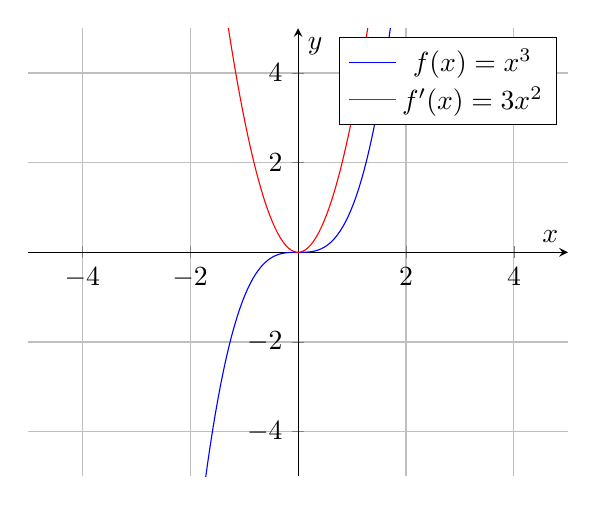
\begin{tikzpicture}
        \begin{axis}[
            xmin = -5,
            ymin = -5,
            xmax = 5,
            ymax = 5,
            xlabel = $x$,
            ylabel = $y$,
            axis lines = middle,
            grid
        ]
        
        \addplot[blue, domain=-5:5,samples=200] {x * x * x};
        \addlegendentry{$f(x) = x^3$};
        
        \addplot[red, domain=-5:5,samples=200] {3 * x * x};
        \addlegendentry{$f'(x) = 3x^2$};
        
        \end{axis}
    \end{tikzpicture}
    \caption{Graphe de $f(x) = x^3$ et de la dérivée $f'(x) = 3x^2$}
    \label{fig:x_cubed}
\end{figure}

De même, si on considère les extrema de la fonction sur un intervalle fermé, alors la dérivée n'est pas définie aux bords de celui-ci. Il nous faut alors regarder, en plus de ces points critiques, les valeurs de la fonction aux bords de l'intervalle. Par exemple, si on considère la fonction $f(x) = x^3 - x^2$ sur le domaine $[-1, 3]$, alors les points où sa dérivée s'annule sont
\begin{equation}
f'(x) = 3x^2 - 2x = 3x\left(x-\frac{2}{3} \right) = 0 \implies x = 0, \frac{2}{3}
\end{equation}
Puisque $f'$ est une fonction quadratique, une rapide étude de son signe nous donne que 
\begin{table}[H]
    \centering
    \begin{tikzpicture}
        \tkzTabInit{$x$/1, $f'(x)$/1}{$-1$, $0$, $\frac{2}{3}$, $3$}
        \tkzTabLine{, + , z, -, z, +, }
    \end{tikzpicture}
    \caption{Tableau de signe de $f'(x) = 3x^2 - 2x$}
    \label{tab:signe_derivee}
\end{table}
Ainsi $f'$ change de signe en $x = 0$ et en $x = \frac{2}{3}$, ce qui en fait des extrema locaux. Or, il serait faux de croire que ce sont des extrema globaux de $f$ sur $[-1, 3]$, car
\begin{equation}
f(0) = 0 < f(3) = 18 \quad \textrm{et} \quad f\left(\frac{2}{3}\right) = -\frac{4}{27} > f(-1) = -2
\end{equation}
Ainsi, il est crucial de ne pas oublier le domaine sur lequel on étudie notre fonction.

% Pour un maximum, la dérivée passe d'une valeur positive à une valeur négative, donc est décroissante. Or, une fonction décroissante peut être étudiée grâce à... la dérivation. On peut alors redériver la fonction dérivée, et on obtient alors la \emph{dérivée seconde}~:
% \begin{boxdef}[Dérivée seconde, $n$-ième]
% Soit $f : D \to \mathbb{R}$, dérivable en $x \in D$. Si $f' : D' \to \mathbb{R}$ est dérivable en $x$, on dit que $f$ est deux fois dérivable en $x$, et on note
% \[
% (f')'(x) = f''(x)
% \]
% Plus généralement, si $f$ est $n$-fois dérivable en $x$, on note la $n$-ième dérivée de $f$ en $x$ par $f^{(n)}(x)$.
% \end{boxdef}

% La dérivée seconde nous permet ainsi d'exprimer le résultat suivant~:
% \begin{boxthm}
% Soit $f : D \to \mathbb{R}$ une fonction 2 fois dérivable en $x \in D$. Alors
% \begin{itemize}
%     \item Si $f'(x) = 0$ et $f''(x) < 0$, alors $f$ admet un maximum local en $x$
%     \item Si $f'(x) = 0$ et $f''(x) > 0$, alors $f$ admet un minimum local en $x$
% \end{itemize}
% Si $f'(x) = f''(x) = 0$, alors on ne peut rien conclure (e.g. pour $f(x) = x^4$, $x = 0$ est un minimum, alors que pour $g(x) = x^3$, $x = 0$ n'est pas un extremum).
% \end{boxthm}